%----------------------------------------------------------------------------
\chapter{Irodalmi áttekintés}
%----------------------------------------------------------------------------

\section{Mobil robotok irányítása}
A mobil robotok irányítása alapvető szerepet játszik az autonóm rendszerek hatékony működésében. Az autonóm mobil robotok  alkalmazási területeik két részre bonthatók, az egyik az olyan feladatok, amelyek nagy precizitást igényelnek és egy embernél gyorsabban, pontosabban szükségesek elvégezni, a másik a könnyen autómatizálható feladatok, ahol robotok alkalmazásával jelentős költségmegtakarítás érhető el. Például:

\begin{itemize}
    \item \textbf{Logisztika}: Raktári robotok optimalizálják az áruk szállítását, csökkentve az emberi erőforrás szükségletét és növelve a hatékonyságot.
    \item \textbf{Egészségügy}: Autonóm robotok biztosítják a steril környezetet és az időérzékeny anyagok szállítását kórházakban.
    \item \textbf{Mezőgazdaság}: Robotok segítenek a precíziós gazdálkodásban, például a növények állapotának monitorozásában vagy a gyomirtásban.
\end{itemize}

Az autonóm mobil robotok sikere nagyban függ a vezérlési rendszer minőségétől. Egy hatékony irányítórendszer:
\begin{enumerate}
    \item \textbf{Pontosan vezérli a robot mozgását} a megadott pályán.
    \item \textbf{Akadályokat kerül el biztonságosan}, az emberi és környezeti tényezőket figyelembe véve.
    \item \textbf{Döntéseket hoz valós időben} a változó környezetben.
    \item \textbf{Energiahatékony} működést biztosít, ami különösen fontos akkumulátorról működő rendszerek esetén.
\end{enumerate}

A mobil robotok irányítása különösen bonyolult, mivel figyelembe kell venni:
\begin{itemize}
    \item a robot kinematikai és dinamikai modelljét,
    \item a környezeti bizonytalanságokat, például dinamikus akadályokat,
    \item a rendszer korlátait, mint például a szenzorok pontosságát és a robot fizikáját.
\end{itemize}

\section{Robotok mechanikai felépítése}
Robotok mechanikai felépítésük alapján kétféle csoportra oszthatók: térbeli mozgásra képes és mozgásra nem képes alappal rendelkezők. A fix alaphoz kötött robotok geometriai felépítése leírható merev testek (links) és csuklók (joints) kapcsolatainak sorával, melyek egy adott munkatérben képesek mozogni. A mozgó alappal rendelkező robotok a térben helyet tudnak változtatni. Mechanikai szempontból egy vagy több merev testből állhatnak, melyekhez csatlakozik egy elmozdulásra képes rendszer például kerekek. \cite{siciliano2010robotics}

\subsection{Mobil alappal rendelkező robotok}
Mobil robotok tovább csoportosíthatók kerekekkel (vagy valamilyen elforduló mechanizmussal) vagy lábakkal mozgó osztályokra. Továbbiakban a kerekekkel rendelkező robotokról lesz szó, mivel ez az osztály lényeges a diplomamunka szemszögéből. Az ilyen robotok különféle kerék mechanizmusokkal szerelhetők fel, ahogyan a képen (\refstruc{fig:wheels}) is látható:
\begin{figure}[!ht]
    \centering
    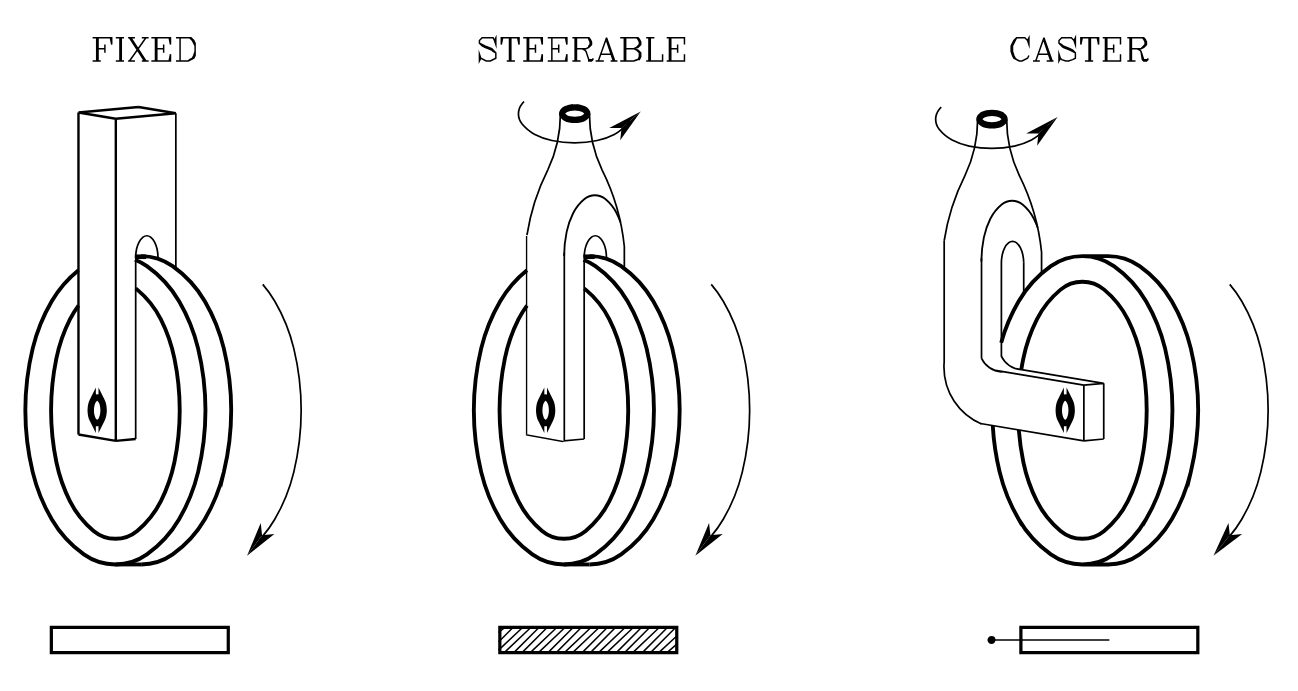
\includegraphics[width=150mm, keepaspectratio]{figures/021_wheels.png}
    \caption{Kerék mechanizmusok \cite{siciliano2010robotics}}
    \label{fig:wheels}
\end{figure}

\begin{itemize}
    \item \emph{Fix kerekek (fixed)}: csak irányban forognak (előre-hátra), nem képesek elfordulni oldalirányban. Általában meghajtott kerekek tartoznak ide, amelyek a robot hajtását biztosítják, például egy autó hátsó tengelyére szerelt kerekek. A robot bázisához mereven csatlakoznak és saját tengelyük körül forognak, amely ortogonális a kerék síkjára.\cite{siciliano2010robotics}
    \item \emph{Kormányozható (steerable) kerekek}: oldalirányban elfordíthatók, a haladási irányuk megváltoztatható, például autó első tengelyén lévő kerekek. A robot bázisához egy csuklóval csatlakoznak, mely lehetővé teszi a kerekek elfordulását, illetve erre merőleges saját tengellyel rendelkeznek (szintén merőleges a kerék síkjára), melyek körül forognak.\cite{siciliano2010robotics}
    \item \emph{Szabadonfutó (bolygó/caster) kerekek}: hasonló mechanikai csatlakozással rendelkeznek, mint az irányítható kerekek, azonban a robot bázisához való csatlakozásuknál található tengely körül szabadon fordulnak el, például irodai székek vagy bevásárló kocsi kerekei. A vertikális tengely nem metszi a kerék elfordulási tengelyét hanem egy "offset" távolságra helyezkedik el. Ezek a kerekek mechanikai stabilitásban segítik a robot bázist.\cite{siciliano2010robotics}
\end{itemize}

\subsection{Mobil kerekes robotok kinematikai modellje}
Kétféle csoportosítás különíthető el: holonomikus (nem tud mozogni a sík bármelyik irányában) és omnidirekcionális (tetszőleges irányba képes mozogni). Omnidirekcionális robotok mecanum (másik nevén svéd) kerekekkel (\refstruc{fig:023_omni_wheel}) felszerelt robotok, melyek több forgó alkatrésszel rendelkeznek, a kerék kerületen mentén független elfordulni képes görgők vannak amik segítségével oldalazó mozgást is végezhet a kerék tengelyével párhuzamosan. \cite{siciliano2010robotics} \cite{ros2_control_docs}

\begin{figure}[!ht]
    \centering
    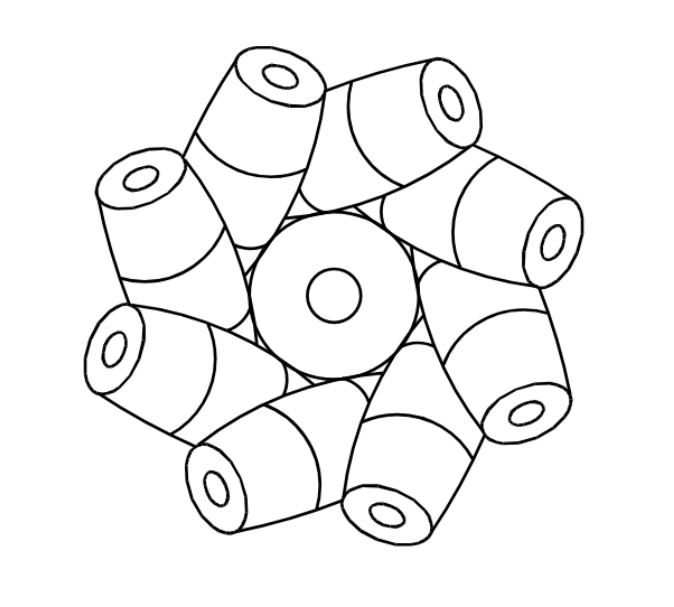
\includegraphics[width=75mm, keepaspectratio]{figures/023_omni_wheel.png}
    \caption{Mecanum kerék \cite{siciliano2010robotics}}
    \label{fig:023_omni_wheel}
\end{figure}

A dolgozatban vizsgált robotmodellek holonomikusak. Több fajta (előző pontban tárgyalt) kerék elrendezéssel hozható létre ilyen robotmodell. Klasszikusan a tricikli modell (\refstruc{fig:024_tricikli_car}), amely egy tengelyen két együttesen meghajtott kerékkel rendelkezik és egy kormányzott kerékkel. Az autókhoz hasonló modellek négy kerékkel (\refstruc{fig:024_tricikli_car}) ahol ebből kettő meghajtott és kettő kormányozható, vagy kettő egyszerre kormányozható és meghajtott plusz kettő stabilitásban asszisztáló fix kerékkel. Differenciál hajtású mobil robotok (\refstruc{fig:025_diff_model}) is a holonomikus robotok közé tartoznak, melyek két függetlenül meghajtott kerékkel és egy vagy több szabadon elforduló kerékkel szerelnek fel.  \cite{siciliano2010robotics} \cite{ros2_control_docs}

\begin{figure}[!ht]
    \centering
    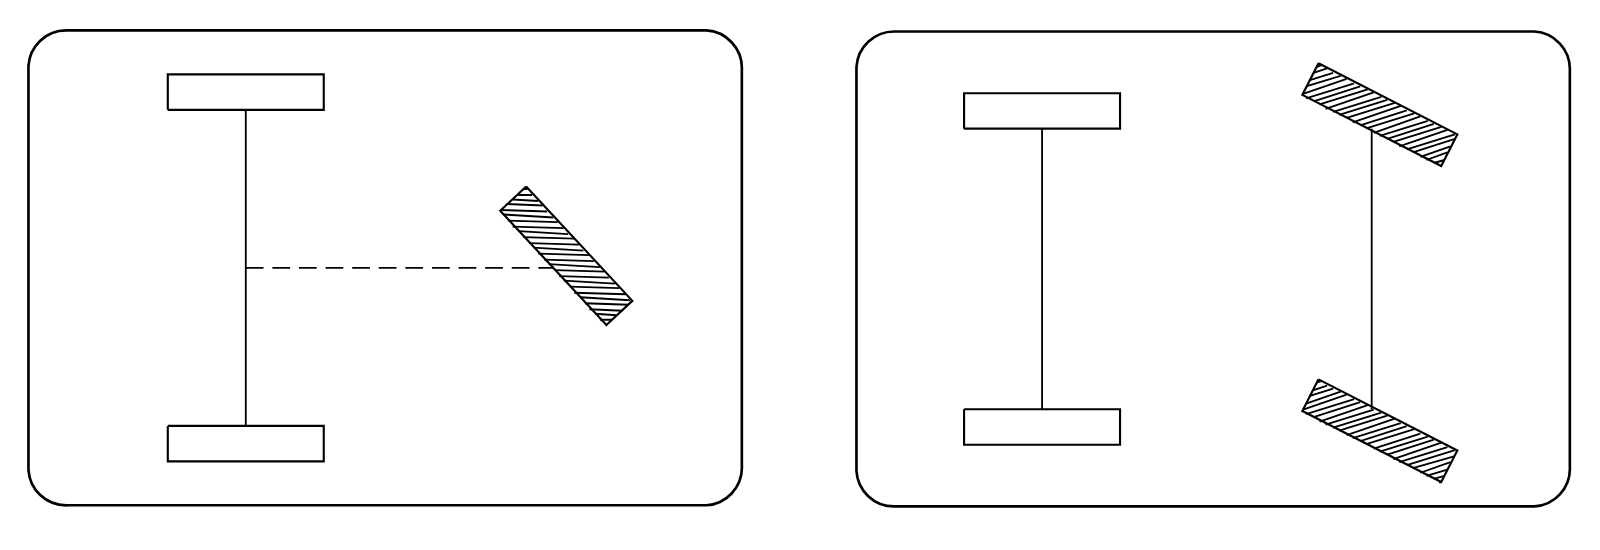
\includegraphics[width=150mm, keepaspectratio]{figures/024_tricikli_car.png}
    \caption{Tricikli és autó modellek \cite{siciliano2010robotics}}
    \label{fig:024_tricikli_car}
\end{figure}

\subsection{Differenciál hajtású robotok}
TODO: források
% Siegwart, R., Nourbakhsh, I. R., & Scaramuzza, D. (2011). Introduction to Autonomous Mobile Robots. MIT Press.
% Bekey, G. A. (2005). Autonomous Robots: From Biological Inspiration to Implementation and Control. MIT Press.

A diplomamunka során használt robotok közül mindegyik ebbe a kategóriába esik. Két szeparáltan meghajtott kerekének köszönhetően egyhelyben képesek megfordulni. A forgás tengelye a két kerék tengelyének közzéppontja. A passzív caster kerék vagy kerekek a stabilitásban segítenek, ezek lekövetik a robot mozgását. Ugye egy sík három pontból már felírható ezért a robot statikai egyensúlya nem jelent problémát, amíg a tömegközéppont vetülete a mozgás síkjára a három vagy több kerek talajjal való találkozási pontjainak egyenes szakaszokkal összekötő polinom belsejében marad. Mint mobil robot a differenciál hajtású szerkezetek munkatere virtuálisan végtelen, ha a munkateret a környezet egy altereként értelmezzük. A valóságban természetesen előjönnek olyan korlátok, mint a robot fizikai kiterjedése és a környezetben lévő akadályok relatív mérete és pozíciója. Természetesen itt sík felületet feltételezve (és kizárva lépcsőket, lifteket stb.) Mint nem omnidirekcionális robotmodell a lokális elmozdulására esnek korlátok. Nem tud rögtön a hajtott kerekek tengelyére merőleges irányába elmozdulni, ehhez szükséges fordulnia. De képesnek tekinthető bármely pozíciót felvenni csak nem rögtön. Ez úgy is kifejezhető, hogy a robot szabadsági fokainak száma alacsonyabb, mint a pozíciót leíró vektor változói. \cite{siciliano2010robotics} \cite{ros2_control_docs}

\begin{figure}[!ht]
    \centering
    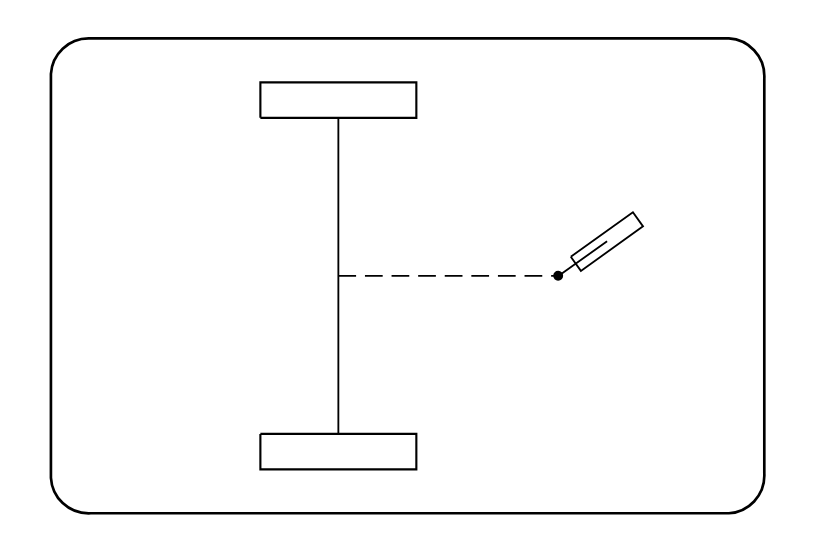
\includegraphics[width=75mm, keepaspectratio]{figures/025_diff_model.png}
    \caption{Differenciál hajtású robot modell \cite{siciliano2010robotics}}
    \label{fig:025_diff_model}
\end{figure}

A differenciál hajtású robotok számos előnnyel rendelkeznek más mechanikai felépítésekkel szemben, amelyek közül az egyik legkiemelkedőbb a szerkezet egyszerűsége. A két különálló hajtott kerék és a passzív támasztó kerekek kombinációja mechanikailag egyszerű és költséghatékony megoldást kínál, amely csökkenti mind a gyártási, mind a karbantartási költségeket. Ez a kialakítás különösen előnyös az oktatási és kutatási célú alkalmazásokban, ahol a költséghatékonyság kiemelt szempont.

Ezen kívül a differenciál hajtású robotok manőverezési képességei kimagaslóak. A két hajtott kerék lehetővé teszi, hogy a robot helyben forduljon, azaz nulla sugarú fordulást hajtson végre, ami rendkívül hasznos szűk helyeken történő navigáció során. Ez a képesség különösen beltéri környezetben, például raktárakban, laboratóriumokban vagy otthoni robotikai alkalmazásokban biztosít jelentős előnyt.

Energiafelhasználásuk szintén kedvező. A differenciál hajtású rendszerek egyszerű hajtásmechanizmusa kevésbé energiaigényes, mint a komplexebb robotmechanizmusok, például a lánctalpas vagy az omnidirekcionális rendszerek. Emellett stabilitásuk is kiemelkedő: a három vagy több támasztópont miatt a robot mozgása stabil, feltéve, hogy a súlypontja a támasztópontok által határolt területen belül helyezkedik el.

Ugyanakkor vannak hátrányai is ezeknek a rendszereknek, különösen más, fejlettebb mechanizmusokkal összehasonlítva. A differenciál hajtású robotok nem omnidirekcionálisak, azaz nem képesek azonnal bármely irányba mozogni. Mozgásuk gyakran több lépést igényel, mivel a hajtott kerekek tengelyére merőleges irányú elmozduláshoz először el kell fordulniuk. Ez korlátozza mobilitásukat dinamikus és változó környezetekben, ahol gyors irányváltásokra van szükség. Ez kihívást nyújt különböző szabályzók tervezésekor, használatakor.

Ezenkívül a differenciál hajtású robotok mozgása sík terephez kötött, ami akadályokkal vagy egyenetlen talajjal tarkított környezetben problémát jelenthet. Fizikai korlátok akadályozhatják nehezebb tárgyak szállításában, szemben például a lánctalpas robotokkal. Továbbá, csúszós felületeken, például koszos vagy nedves padlón, fordulás közben a kerekek megcsúszhatnak, ami pontatlan manőverezést eredményezhet. Ezek olyan problémák, amik kezelhetőek, de fontos megjegyezni, hogy el nem hanyagolhatók. Például nehezebb terhek szállításánál a kerekek terhelése nőhet, ezért opcióként kell tekinteni több bolgyó kerék beépítésére. A talaj és hajtott kerekek közötti súrlódás növelése érdekében a kerekek anyagát és mintázatát is figyelembe kell venni, illetve nem hanyagolható el a gondolat és igény a szoftveres kerék kicsúszás detektálásra és abból eredő korrigálásra, aminek szintén megvannak a maga eszközei, korlátai.

Összességében a differenciál hajtású robotok egyszerűségük, hatékonyságuk és könnyű kezelhetőségük miatt kiváló választást jelentenek számos alkalmazási területen, azonban érdemes figyelembe venni a mobilitásukból és környezeti korlátaikból adódó hátrányokat is. Egy tipikus példa a TurtleBot\footnote{TurtleBot: \url{https://www.turtlebot.com/}}sorozat, amelynek egyszerű és hatékony kialakítása ideális oktatási célokra és beltéri autonóm navigációra. Diplomamunka során három differenciál hajtású robotmodellt használtam. Ebből kettő TurtleBot hármas szérájából a waffle és burger model és egy méretében nagyobb robotmodellt, melynek fejlesztésén munkahelyemen dolgozok. Ezekre később részletesen kitérek, viszont itt szeretnék egy rövid ismertetést írni a TurtleBot-okról.

TODO: képek (tb3 burger waffle)

A TurtleBot egy alacsony költségű, személyes robotkit, amely nyílt forráskódú szoftverrel érkezik, és kifejezetten oktatási, kutatási, hobbi és prototípusfejlesztési célokra tervezték. A diplomamunkám során a TurtleBot 3-as verzióját használtam, azon belül is a Burger és Waffle modelleket. A TurtleBot 3 célja, hogy jelentősen csökkentse a robotplatform méretét és árát, miközben megőrzi a funkcionalitást és minőséget, valamint lehetőséget biztosítson a bővíthetőségre. A robot platformja rugalmasan alakítható át a mechanikai részek újraszerkesztésével (akár otthoni 3D nyomtatott alkatrészekkel) és különböző szenzorok, mikrovezérlővel vagy elektronika hozzáadásával.

TODO: forrás: TurtleBot Inventors Tell Us Everything About the Robot (IEEE Spectrum, By Evan Ackerman, 26 Mar 2013)
https://spectrum.ieee.org/interview-turtlebot-inventors-tell-us-everything-about-the-robot

\subsection{Differenciál hajtású robotok mozgásegyenletei}
TODO: források
% Roland Siegwart, Illah R. Nourbakhsh, Davide Scaramuzza
% Introduction to Autonomous Mobile Robots
% MIT Press, 2011.
% Autonomous Robots: From Biological Inspiration to Implementation and Control
% MIT Press, 2005.

A differenciál hajtású robotok mozgását a kinematikai modelljük írja le, amely az egyes kerekek sebességének és a robot általános mozgási paramétereinek kapcsolatát adja meg. Ezeket a mozgásegyenleteket arra használjuk, hogy a robot mozgását leírjuk, vagy vezérlési parancsokat generáljunk a kívánt mozgás eléréséhez. A mozgásegyenletek alapja, hogy a robot egy síkon mozog, két hajtott kerékkel és esetleg további szabadonfutó kerekekkel van felszerelve.

\begin{figure}[!ht]
    \centering
    \includesvg[scale=1.2]{figures/022_diff_drive.svg}
    \caption{Differenciál hajtású robot 2 dimenzióban \cite{ros2_control_docs}}
    \label{fig:022_diff_drive}
\end{figure}

A \refstruc{fig:022_diff_drive} jelölései a következők. A $v_{right}$ és $v_{left}$ a jobb, illetve bal oldali kerék kerületi lineáris sebessége. Ez a sebesség a kerék érintkezési pontján mért, a kerék síkjára merőleges érintőirányú sebesség, amely meghatározza, hogy a kerék milyen gyorsan halad előre (vagy hátra) a talajon. Az SI mértékegységük $\mathrm{m/s}$. A kerületi sebességek ($v_{right}$ és $v_{left}$) közvetlenül kapcsolódnak a kerék forgási sebességéhez, valamint a kerék sugarához az összefüggés $v = \omega r$ alapján, ahol $\omega$ a forgási sebesség (kerekeké), $r$ pedig a kerék sugara. $v_x$: a robot bázispontjának lineáris sebessége a robot $x$ tengelye mentén. Ez a robot középpontjára vonatkozó előrehaladási sebesség, amely a két kerék sebességének átlaga alapján számítható ki. Az SI mértékegysége $\mathrm{m/s}$.
$\omega_z$: a robot szögsebessége a $z$ tengely körül (amely a síkból felfele mutat). Ez a robot forgási sebessége, amely a két kerék közötti sebességkülönbségen alapul. Az SI mértékegysége $\mathrm{rad/s}$. $w$: a két hajtott kerék tengelyei közötti távolság (nyomtáv). Ez egy statikus paraméter, amely a robot mechanikai kialakításától függ. Az SI mértékegysége $\mathrm{m}$. Ezek a változók szolgálnak a robot aktuális mozgásának modellezésére. S az alábbi mozgásegyenletekkel írják le a robot mozgását:
\begin{align}
    v_{x}      & = \frac{v_{right} + v_{left}}{2}, \\
    \omega_{z} & = \frac{v_{right} - v_{left}}{w}, \\
    v_{left}   & = v_{x} - \omega_{z} \frac{w}{2}, \\
    v_{right}  & = v_{x} + \omega_{z} \frac{w}{2}.
\end{align}

Az egyenletek értelmezése alapján $v_{left}$ és $v_{right}$ a bal és jobb oldali hajtott kerekek sebessége, amelyek a robot általános mozgásának eléréséhez szükségesek. Az egyenletek tehát lehetővé teszik a robot aktuális mozgásának leírását, valamint a kívánt mozgási paraméterek alapján a keréksebességek kiszámítását. Ezek az összefüggések elengedhetetlenek a robot vezérléséhez és navigációjához, valamint az autonóm mozgás tervezéséhez. A diplomamunka során használt robotok irányítása az $v_x$ és $\omega_z$ paraméterek segítségével oldaható meg. A szablyzónak ezeket az értékeket szükséges meghatározni, a mozgásegyenletek segítségével pedig a motorvezérlő vagy szimulációban differenciál hajtást biztosító pluigin feladatkörébe tartozik az egyes kerekek megfelelő sebességének ($v_{right}$ és $v_{left}$) beállítása.

\section{Robotok szabályozása}
A szabályozás kulcsfontosságú a mobil robotok működésében, mivel biztosítja a robot mozgásának stabilitását és pontosságát. Egy autonóm robotnak képesnek kell lennie arra, hogy különböző környezeti feltételek között is megbízhatóan navigáljon, miközben leköveti a kívánt pályát. A szabályozás feladata, hogy a robot kerekének sebességét és irányát dinamikusan módosítsa a kívánt mozgás eléréséhez. Az optimális szabályozás nélkül a robot mozgása instabillá válhat, például csúszás vagy pontatlan kanyarodás léphet fel. Egy jól működő szabályozási rendszer képes kompenzálni a szenzorokból és aktuátorokból származó hibákat, például a kerékcsúszást vagy a zajos pozícióadatokat. A differenciál hajtású robotok esetében a szabályozás különösen fontos, mivel a két hajtott kerék sebességének összehangolása határozza meg a haladási és forgási mozgásokat. A szabályozás lehetővé teszi a robot számára, hogy gyorsan reagáljon a környezet változásaira, például mozgó akadályok elkerülésére. Emellett a szabályozás biztosítja a robot energiahatékonyságát, optimalizálva a hajtáshoz szükséges erőforrásokat. A komplexabb környezetekben, például dinamikus akadályok vagy szűk helyek esetén, a szabályozási algoritmusok teszik lehetővé a robot biztonságos és precíz működését.

\subsection{PID szabályzó}
A PID szabályzó (arányos, integráló, deriváló szabályozó) az egyik legelterjedtebb módszer a vezérlőrendszerekben. Az arányos elem a jelenlegi hiba arányában reagál, az integráló elem a múltbeli hibák összegét veszi figyelembe, míg a deriváló elem a hiba változásának sebességére reagál. Ez a kombináció lehetővé teszi a szabályzó számára, hogy stabilan és pontosan kövesse a kívánt értékeket \cite{astrom_feedback}.

A PID szabályozó különösen hasznos lehet a robotok sebességszabályozásában, például differenciálhajtású robotok esetén, ahol a kerekek forgási sebességét kell koordinálni az egyenes vonalú mozgás vagy a fordulás érdekében. Mint szabályzó nagyon egyszerű útvonalkövetésnél is használható, ám nyilvánvalóak korlátai. A legelterjedtebb használata motorvezérlőknél jelenik meg, ahol alacsony szinten kell vezérlési feladatokat ellátni. Itt egyszerűsége és gyorsasága nagy előnyt jelent \cite{siciliano_springer_handbook}.

Ennek ellenére a PID szabályozó egyszerűsége egyben a korlátja is. Nem képes kezelni komplex, nemlineáris rendszereket vagy többdimenziós optimalizációs problémákat. Emellett a szabályozó paramétereinek manuális hangolása időigényes lehet, és a szabályzó teljesítménye jelentősen csökkenhet, ha a rendszer dinamikája változik \cite{ogata_modern_ce}.

\subsection{PID és az MPC között}
A PID szabályozó és a model prediktív szabályozás (MPC) között számos olyan szabályozási módszer létezik, amelyek képesek hatékonyan kezelni a robotok sebességvezérlését, különösen útvonalkövetési feladatok esetén. Ezek közé tartozik például a Dinamikus Ablak Alapú (Dynamic Window Approach, DWA) szabályozó \cite{fox_dynamic}.

A DWA egy lokális szabályozási technika, amely az akadálykerülésre és a kívánt sebesség elérésére koncentrál azáltal, hogy egy adott időablakon belül optimalizálja a robot mozgását. Ez a szabályozó különösen jól alkalmazható beltéri robotok navigációjára, ahol az akadályok dinamikusak és a navigációs tér szűk. Bár a DWA hatékony, korlátai közé tartozik, hogy csak lokális optimumokat talál, és nem képes globális optimalizációs problémák kezelésére. Ami természetesen nem jelent problémát, mert egy konvencionális autonóm navigációnál, hiszen itt a szabályzó feladata tényleg a robot környezetében alkalmazott. Jól alkalmazható egy frekventált globális útvonal újratervezést implementáló roboton \cite{siciliano_springer_handbook}.

Más, hasonló szabályozók, mint például a potenciálmező-alapú szabályozók vagy az állapotvisszacsatolásos szabályozók, szintén széles körben használatosak. Ezek gyakran a robot kinematikájának és dinamikájának egyszerűsített modelljére támaszkodnak, és hatékonyak lehetnek egyszerűbb környezetekben, de korlátozottak, amikor komplex akadályok vagy nemlineáris dinamikák lépnek fel \cite{latombe_robot}.

\subsection{Korlátok és igények a modern szabályozásban}
A hagyományos szabályozási módszerek, mint a PID vagy a DWA, gyakran nem tudnak megbirkózni az autonóm rendszerek összetett követelményeivel. Nemlineáris dinamikák, változó környezeti feltételek, valamint a rendszerek fizikai és működési korlátai olyan kihívásokat jelentenek, amelyeket ezek a szabályozók nem tudnak hatékonyan kezelni \cite{rawlings_model}.

A modern robotikai rendszerek egyre inkább igénylik az optimalizációs célok és komplex korlátok kezelésére képes szabályozási technikákat. A model prediktív szabályozás (MPC) ebben az értelemben kiemelkedő megoldást nyújt, mivel képes előrejelezni a rendszer viselkedését és optimalizálni a vezérlési parancsokat a jövőbeli állapotok alapján. Az MPC lehetőséget biztosít arra, hogy dinamikusan alkalmazkodjon a környezeti változásokhoz \cite{rawlings_model}.

\section{Model prediktív szabályozás (MPC)}
TODO: hivatkozások
% Camacho, E. F., & Bordons, C. (2007). Model Predictive Control. Springer.
% Mayne, D. Q., Rawlings, J. B., Rao, C. V., & Scokaert, P. O. M. (2000). Constrained Model Predictive Control: Stability and Optimality. Automatica, 36(6), 789-814.
% Maciejowski, J. M. (2002). Predictive Control with Constraints. Prentice Hall.

A model prediktív szabályozás (MPC) egy olyan irányítási módszer, amely a vezérlési feladatokat egy adott időhorizonton belüli optimalizálási problémaként kezeli. Az MPC alapötlete az, hogy a vezérlő a rendszer jövőbeli állapotainak előrejelzésére támaszkodva határozza meg az aktuális vezérlési parancsokat. Ez a megközelítés különösen hatékony dinamikus, nemlineáris és változó környezetekben, ahol a hagyományos szabályozók nehezen alkalmazhatók. Az MPC a rendszer viselkedésének leírására egy matematikai modellt használ, amely jellemzi a rendszer dinamikáját (pl. differenciálegyenletek vagy állapotegyenletek formájában). Megold egy optimalizálási problémát egy adott időhorizonton, amely során minimalizál egy költségfüggvényt (pl. távolság a célponttól). Képes kezelni a rendszer fizikai és működési korlátait, például sebesség- vagy gyorsulási határokat. Az optimalizáció mindig az aktuális állapotból indul, és az időhorizont minden iterációban előre gördül egy megadott időegységgel.

Diszkrét időben egy nemlineáris, determinisztikus rendszernél ez azt jelenti, hogy minden $k$ időpillanatban, meghatározunk egy $N$ időpillanattal (horizont) előre mutató beavatkozó jel sorozatot a rendszer jelenlegi $x_k$ állapotához: $\mathrm{x_k \rightarrow [u_{k+1}, u_{k+2}, ... u_{k+i}, ... u_{k+N}]}$. Majd a meglévő modellt ($\mathrm{x_{k+1} = f(x_k, u_k), y_k = g(x_k)}$) felhasználva, minden beavatkozó jel sorozathoz, kapunk az időhorizonton $\mathrm{y_{k,...,k+N}}$ kimenet értékeket. Ezekből felírható az optimalizálási probléma, amire majd specifikusan az MPPI-nél térek ki. Itt azt szeretném kiemelni és szemléltetni, hogy a jelek sorozatai lehetőséget nyújtanak költségfüggvény részletes paraméterezésére. Opciót biztosít, hogy a beavatkozó jeleknél különféle limiteket állítsunk be, példuál büntetve a túl magas vagy alacsony értékeket. Ugyanez a kimeneti oldalról is elvégezhető. Robotikai alkalamzásnál maradva, az $u_k$ beavatkozó jelnek a sebességet vesszük, akkor a költségfüggvényben leírhatóak gyorsulás korlátok. Sebességekből a modell szerint a horizonton előrevetített pályát számolva annak eltérését lehet büntetni a tervezett útvonaltól.

Az MPC alkalmazása számos területen kiemelkedően hasznos. A robotikában például az MPC alapú vezérlés lehetővé teszi a dinamikus környezetben történő pályakövetést és akadálykerülést. Ez különösen fontos olyan autonóm rendszerek esetén, ahol a robotoknak gyorsan kell reagálniuk a változó körülményekre, miközben biztonságosan és hatékonyan teljesítik a feladataikat.

Az autonóm járművek irányításában az MPC széles körben alkalmazható. A járművek mozgásának optimalizálása érdekében az MPC figyelembe veszi a biztonsági és energiahatékonysági szempontokat. Az előrejelzés alapú vezérlés lehetővé teszi, hogy a jármű elkerülje az ütközéseket és optimális útvonalakat válasszon, miközben a fogyasztást is minimalizálja.

A folyamatirányítás területén az MPC a gyártási folyamatok vezérlésének egyik kulcstechnológiája. Az ipari rendszerek optimalizációja során az MPC csökkenti az energia- és anyaghasználatot, miközben biztosítja a termelés folytonosságát és a minőségi követelmények teljesítését. Az ilyen rendszerekben az MPC használata különösen akkor előnyös, ha a működés során változó feltételekhez kell igazítani a folyamatparamétereket.

Ezek az alkalmazási példák jól mutatják, hogy az MPC mennyire sokoldalú eszköz, amely különböző területeken is képes a szabályozási problémák megoldására. Az optimalizációs képességei és a valós idejű adaptáció lehetőségei miatt az MPC számos modern irányítórendszer alapját képezi.

\section{MPPI}
TODO: nav2-es hivatkozás
% https://roscon.ros.org/2023/talks/On_Use_of_Nav2_MPPI_Controller.pdf
%https://ieeexplore.ieee.org/abstract/document/7487277
% -> https://sci-hub.se/10.1109/icra.2016.7487277
Az Model Predictive Path Integral (MPPI) szabályozó egy modern, mintavétel-alapú modell prediktív szabályozási algoritmus, amelyet komplex, nemlineáris rendszerek irányítására fejlesztettek ki. Az MPPI az optimalizációs és információelméleti módszerek kombinációján alapul, és hatékonyan alkalmazható valós idejű feladatok megoldására, ahol a hagyományos szabályozók nem biztosítanak elegendő rugalmasságot. Az MPPI a jövőbeli rendszerállapotok előrejelzésével és az ezekhez tartozó költségek minimalizálásával dolgozik. Az algoritmus véletlenszerűen generált irányítási pályákon keresztül vizsgálja a rendszer dinamikáját, majd az optimális pályát a költségfüggvény alapján választja ki.

\begin{enumerate}
    \item \textbf{Zaj hozzáadása az előző optimális pálya irányítási parancsaihoz:}
    Az algoritmus véletlenszerű zajt ad az előzőleg kiszámított optimális irányítási parancsokhoz. Ez lehetővé teszi a lehetséges irányítási pályák felfedezését, és segít elkerülni a lokális optimumokat.

    \item \textbf{A dinamikai modell alkalmazása és a pályák szimulációja:}
    A zajjal módosított irányítási parancsok alapján az algoritmus szimulálja a rendszer dinamikáját, és meghatározza a lehetséges pályák sorozatát (ún. rollout trajektóriák). Ezek a trajektóriák a rendszer viselkedésének lehetséges jövőbeli állapotait modellezik.

    \item \textbf{A trajektóriák értékelése költségfüggvényekkel:}
    Minden trajektóriához hozzárendel egy költségértéket az adott költségfüggvény alapján, amely figyelembe veszi például a pályán maradást, a kívánt sebességet és az irányítás hatékonyságát. Az alacsonyabb költségű pályák jobban preferáltak.

    \item \textbf{Új optimális irányítási parancssorozat kiszámítása:}
    Az algoritmus az értékelt trajektóriák súlyozott átlaga alapján frissíti az irányítási parancsokat. Az alacsony költségű trajektóriák nagyobb súlyt kapnak, így az új parancsok az optimális pálya elérését célozzák.

    \item \textbf{Az első irányítási parancs végrehajtása és az algoritmus ismétlése:}
    Az algoritmus végrehajtja az újonnan kiszámított irányítási parancs első elemét, majd a fennmaradó parancsokat előre tolja az időben. Ezután az egész folyamatot megismétli a következő időlépésre vonatkozóan.
\end{enumerate}

\subsection{Optimalizációs cél}
Az MPPI algoritmus célja az optimális vezérlési jel sorozat (autonóm robot esetében a beavatkozó sebességek) \( \mathbf{u}^* = \{u_0, u_1, \dots, u_{N-1}\} \) meghatározása, amely minimalizálja a rendszer költségfüggvényét és figyelembe veszi a modell dinamikáját. Az optimalizáció célja az alábbi:
\begin{equation}
\mathbf{u}^* = \arg\min_{\mathbf{u}} \mathbb{E}_P \left[ \exp\left(-\frac{1}{\lambda} S(\tau)\right) \right],
\end{equation}

ahol:
\begin{itemize}
    \item \( \mathbb{E}_P \): a rendszer dinamikája szerinti várható érték,
    \item \( S(\tau) \): az adott pálya költsége, amely:
    \begin{equation}
    S(\tau) = \phi(x_T, T) + \int_{t_0}^T q(x_t, u_t, t) \, dt,
    \end{equation}
    \item \( \phi(x_T, T) \): a végállapot költsége,
    \item \( q(x_t, u_t, t) \): a pillanatnyi költség, amely az állapottól \(x_t\) és a bemenettől \(u_t\) függ.
\end{itemize}

\subsection{Relatív entrópia minimalizálása}
Az MPPI algoritmus a vezérlési eloszlást \( Q(u) \) közelíti az optimális eloszláshoz \( Q^*(u) \) a KL-divergencia minimalizálásával:
\begin{equation}
\mathbf{u}^* = \arg\min_{\mathbf{u}} D_{KL}(Q^* \,||\, Q(u)),
\end{equation}

ahol:
\begin{itemize}
    \item \( D_{KL}(Q^* \,||\, Q(u)) \): a relatív entrópia az optimális és az aktuális vezérlési eloszlás között,
    \item \( Q^*(u) \): az optimális vezérlési eloszlás:
    \begin{equation}
    Q^*(\tau) \propto \exp\left(-\frac{1}{\lambda} S(\tau)\right).
    \end{equation}
\end{itemize}

\subsection{Iteratív beavatkozó jel frissítése}
Az MPPI iteratív módon frissíti a vezérlési bemeneteket a következő szabály alapján:
\begin{equation}
\mathbf{u}_j^* = \frac{1}{\Delta t} H^{-1} G \mathbb{E}_P \left[ \exp\left(-\frac{1}{\lambda} S(\tau)\right) \epsilon_j \sqrt{\Delta t} \right],
\end{equation}

ahol:
\begin{itemize}
    \item \( H \) és \( G \): a rendszer dinamikáját leíró mátrixok,
    \item \( \epsilon_j \): véletlenszerű perturbációk,
    \item \( \Delta t \): az időbeli diszkretizáció lépésköze.
\end{itemize}

\subsection{A Módszer Lényege}
Az MPPI vezérlő számos lehetséges pályát generál a nem vezérelt dinamikából kiindulva. Ezeket a pályákat költségfüggvény alapján súlyozza, és a legjobb pályához tartozó vezérlést alkalmazza. A GPU-alapú párhuzamosítás lehetővé teszi, hogy az MPPI valós időben (például 60 Hz-en) optimalizálja a vezérlést, még komplex rendszerek esetében is. Az MPPI algoritmus előnyei közé tartozik, hogy:
\begin{itemize}
    \item képes nemlineáris, nem differenciálható költségfüggvények kezelésére,
    \item valós időben generál új pályákat és viselkedéseket,
    \item robusztus a rendszer dinamikájának pontatlanságával szemben.
\end{itemize}

\section{Optimalizáció}
TODO: források
%Boyd, Stephen, and Lieven Vandenberghe. "Convex Optimization."
%Ez a könyv az optimalizáció elméletének alapjait mutatja be, különös hangsúlyt helyezve a konvex problémákra és azok gyakorlati alkalmazásaira.

%Nocedal, Jorge, and Stephen J. Wright. "Numerical Optimization."
%Ez a mű részletesen tárgyalja a gradiens-alapú módszereket, mint a Newton- és kvázi-Newton-módszerek, amelyek kulcsfontosságúak a mérnöki optimalizációban.

%Goldberg, David E. "Genetic Algorithms in Search, Optimization, and Machine Learning."
%A genetikus algoritmusok alapvető kézikönyve, amely heurisztikus megközelítéseket mutat be komplex optimalizációs problémákra.

%Rawlings, James B., and David Q. Mayne. "Model Predictive Control: Theory and Design."
%Ez a könyv az MPC alapelveit tárgyalja, részletes példákkal illusztrálva, beleértve a prediktív szabályozás és optimalizáció kapcsolatát.

%Deb, Kalyanmoy. "Multi-Objective Optimization Using Evolutionary Algorithms."
%A többcélú optimalizációhoz kapcsolódó evolúciós algoritmusokról nyújt mélyreható áttekintést.

%Garcia, Carlos E., and Manfred Morari. "Model predictive control: theory and practice—a survey." Automatica (1982).
%Ez a cikk széles körű áttekintést nyújt az MPC-ről, beleértve annak gyakorlati alkalmazásait és elméleti hátterét.

%Bertsekas, Dimitri P. "Nonlinear Programming."
%Ez a könyv átfogó bevezetést nyújt a nemlineáris optimalizációba, számos algoritmussal és matematikai eszközzel.
Az optimalizáció egy olyan tudományág, amely az optimális megoldások megtalálására törekszik egy adott probléma esetén, meghatározott célfüggvény és korlátozó feltételek figyelembevételével. Számos mérnöki, gazdasági és tudományos probléma igényli az optimalizáció eszközeinek alkalmazását, különösen olyan esetekben, amikor a rendelkezésre álló erőforrások szűkösek, vagy a cél egy rendszer hatékonyságának maximalizálása.

\subsection{Az optimalizáció általános fogalma}
Az optimalizáció alapvetően egy matematikai probléma megoldását jelenti, amelyben egy célfüggvényt minimalizálni vagy maximalizálni kell. Formálisan az optimalizációs probléma általános alakja:
\begin{align}
    \text{Minimalizálandó vagy maximalizálandó: } & f(x), \\
    \text{Feltételek mellett: } & g_i(x) \leq 0, \quad i = 1, \dots, m, \\
    & h_j(x) = 0, \quad j = 1, \dots, p.
\end{align}

Itt $x$ az optimalizálandó változók vektora, $f(x)$ a célfüggvény, $g_i(x)$ a korlátfeltételeket, $h_j(x)$ pedig az egyenletességi feltételeket reprezentálja.

\subsection{Optimalizáció alkalmazása a robotikában}
Az optimalizáció jelentős szerepet játszik a robotikai rendszerek tervezésében és irányításában. Különösen fontos az autonóm rendszerek esetében, ahol az optimalizáció segítségével maximalizálható a navigáció hatékonysága az útvonalak optimalizálásával, minimalizálhatók az energiafelhasználásból és a mozgásvezérlésből eredő költségek, garantálható az akadályok sikeres elkerülése dinamikus környezetekben. Egy konkrét példaként említhető a \textit{Model Predictive Control} (MPC), amely egy prediktív szabályozási technika. Az MPC optimalizációs eljárásokkal valósítja meg a jövőbeli állapotok előrejelzését és a vezérlési parancsok generálását.

\subsection{Optimalizációs algoritmusok}
Az optimalizációs problémák megoldására számos algoritmus áll rendelkezésre, amelyek közül a leggyakrabban alkalmazottak:

\begin{itemize}
    \item \textbf{Gradiens-alapú módszerek}: Például a Newton-módszer és a gradienscsökkenés, amelyek differenciálható célfüggvényeket igényelnek.
    \item \textbf{Heurisztikus módszerek}: Mint a genetikus algoritmusok vagy a részecskeraj-algoritmus, amelyek komplex vagy nem deriválható problémákra alkalmazhatók.
    \item \textbf{Konvex optimalizációs technikák}: Ezek garantáltan találják meg a globális optimumot konvex problémák esetén.
\end{itemize}

\section{Alkalmazott optimalizációs eljárások}
\subsection{Random keresés}
A random keresés (vagy véletlen mintavételezés) egy egyszerű, heurisztikus optimalizációs módszer, amely véletlenszerűen választ ki pontokat a paramétertérből, és ezeket értékeli a célfüggvény alapján.

\subsubsection{Előnyök}
\begin{itemize}
    \item Könnyen implementálható, és nem igényel előzetes ismereteket a célfüggvényről.
    \item Hatékony lehet magas dimenziós térben, ha az optimális pont közel van a véletlen mintákhoz.
    \item Képes elkerülni a lokális optimumok csapdáját.
\end{itemize}

\subsubsection{Hátrányok}
\begin{itemize}
    \item Lassú konvergencia, különösen nagy paramétertér esetén.
    \item Nem garantált, hogy megtalálja a globális optimumot.
\end{itemize}

A random keresés futásideje az értékelendő minták számától függ. A szükséges minták száma exponenciálisan növekedhet a paramétertér dimenziójával, ami korlátozhatja a módszer hatékonyságát nagyobb dimenziók esetén.

\subsection{Grid keresés}
A grid keresés (rács alapú keresés) a paramétertér egyenletes felosztásával próbálja meg meghatározni az optimális pontot. A módszer minden rácsponton kiértékeli a célfüggvényt.

\subsubsection{Előnyök}
\begin{itemize}
    \item Egyszerű implementáció és determinisztikus viselkedés.
    \item Garantáltan megtalálja az optimális pontot, ha elegendő rácspontot használunk.
\end{itemize}

\subsubsection{Hátrányok}
\begin{itemize}
    \item Magas számítási költség a paramétertér dimenziójának növekedésével.
    \item Nem skálázható jól, mivel a rácspontok száma exponenciálisan növekszik a dimenzióval.
\end{itemize}

A futásidő a rácspontok számával arányos, amely $n^d$ formában írható fel, ahol $n$ a pontok száma tengelyenként, $d$ pedig a dimenziók száma. Ez a kombinatorikus robbanás problémájához vezethet.

\subsection{Bayesian optimalizáció}
A Bayesian optimalizáció egy kifinomultabb módszer, amely a valószínűségi modellezést és az akvizíciós függvényeket használja a paramétertér hatékony mintázására.

\subsubsection{Előnyök}
\begin{itemize}
    \item Hatékony kis mintaszám mellett, mivel a minták helyét adaptívan választja meg.
    \item Jól alkalmazható drága célfüggvények esetén.
    \item Képes kezelni nem deriválható és zajos függvényeket.
\end{itemize}

\subsubsection{Hátrányok}
\begin{itemize}
    \item Összetettebb implementáció, és számításigényes lehet a valószínűségi modell frissítése.
    \item Kevésbé hatékony magas dimenziójú problémák esetén.
\end{itemize}

A Bayes optimalizáció futásideje a valószínűségi modell frissítésének költségétől függ, amely a minták számával nő. Magas dimenziók esetén a modell komplexitása korlátozhatja a hatékonyságot.

\section{Frechét-távolság}
A Frechét-távolság egy széles körben alkalmazott metrika, amely két görbe közötti hasonlóság mérésére szolgál. Eredetileg geometriai problémákra fejlesztették ki, de az autonóm robotikában, különösen a mozgástervezési és pályakövetési feladatok során, rendkívül hasznosnak bizonyul. 

A Frechét-távolság két görbe, \( P \) és \( Q \), között a következőképpen definiálható:
\begin{equation}
    d_F(P, Q) = \inf_{\alpha, \beta} \max_{t \in [0,1]} \| P(\alpha(t)) - Q(\beta(t)) \|,
\end{equation}

ahol:
\begin{itemize}
    \item \( P \) és \( Q \): két görbe, amelyek egy-egy pályát reprezentálnak, \( P : [0,1] \to \mathbb{R}^2 \) és \( Q : [0,1] \to \mathbb{R}^2 \).
    \item \( \alpha \) és \( \beta \): folyamatos paraméterezési függvények, amelyek az \( [0,1] \) intervallumot leképezik a görbékre.
    \item \( \| \cdot \| \): az Euklideszi távolság.
\end{itemize}

A definíció szerint a Frechét-távolság minimalizálja azt a maximális távolságot, amelyet két görbe közötti "sétáló pár" tehet meg, miközben mindkét görbét végigjárják. Ezáltal figyelembe veszi a görbék globális geometriáját, nem csupán a pontok közötti páronkénti távolságot, mint például a Hausdorff-távolság.

A Frechét-távolság különösen hasznos autonóm robotok pályakövetési problémáiban, mivel lehetővé teszi a robot által tervezett pálya és a ténylegesen bejárt pálya közötti eltérések mérését. Ez segít a szabályzó értékelésében, mivel figyelembe veszi a görbék globális geometriáját, nem csupán a pontok közötti távolságokat. A metrika robusztus kiértékelést biztosít olyan esetekben is, ahol a görbék eltérő hosszúságúak vagy zajjal terheltek, ami gyakori a valós robotikai rendszerekben. Szóval megmérhetjük, hogy a robot mennyire pontosan követi a tervezett pályát. A kisebb Frechét-távolság jobb követést jelez, mivel a tényleges és a tervezett pálya közötti eltérés minimális.


\section{RMS módszer: Root Mean Squared}
A Root Mean Squared (RMS) módszer egy statisztikai mutató, amely egy adott adathalmaz átlagos négyzetes eltérését méri. Lehetővé teszi a mozgási dinamikák, például gyorsulások vagy sebességek változásának kvantitatív elemzését. Ez a metrika az MPPI szabályzó alkalmazásában kiemelten fontos, hiszen segítségével objektíven értékelhetők a szabályzó által generált vezérlési jelek.

Az RMS kiszámítása az alábbi képlettel történik:
\begin{equation}
    \text{RMS} = \sqrt{\frac{1}{N} \sum_{i=1}^{N} x_i^2},
\end{equation}

ahol:
\begin{itemize}
    \item \( x_i \): az adatsor \( i \)-edik eleme,
    \item \( N \): az adatsor elemeinek száma.
\end{itemize}

Az RMS kiszámításához először az adatsor minden elemét négyzetre emeljük, majd ezek átlagát vesszük, végül pedig az átlagból négyzetgyököt vonunk. Az eredmény egy olyan skálázott érték, amely jól reprezentálja az adatsor tipikus nagyságát.

Az autonóm robotok mozgásának dinamikája szorosan összefügg a gyorsulási jelekkel, amelyek az alábbi módokon értelmezhetők az RMS segítségével: az RMS mutatja, hogy egy adott időtartományban mekkora volt a gyorsulások átlagos nagysága. Ez fontos indikátor a mozgás simaságának megítélésében, következtethetünk arra, hogy a rendszer milyen mértékben van kitéve erőteljes gyorsulási ingadozásoknak, amelyek növelhetik az energiafelhasználást vagy csökkenthetik a robot mechanikai komponenseinek élettartamát, segít a gyorsulási minták jellemző eltéréseinek kiemelésében, amelyek optimalizációs paraméterek finomhangolását indokolhatják.

\subsection{Előnyök és gyakorlati jelentőség}
Az RMS mutató előnye, hogy robusztus és érzékeny az extrém értékekre, ami különösen hasznos autonóm robotok mozgásának elemzésében. Az MPPI szabályzó finomhangolásánál az RMS segít:
\begin{itemize}
    \item A mozgási minták objektív összehasonlításában,
    \item A dinamikai hatások azonosításában és minimalizálásában,
    \item Az optimalizációs paraméterek precíz meghatározásában.
\end{itemize}
